\documentclass{standalone}
\usepackage{tikz}

\begin{document}

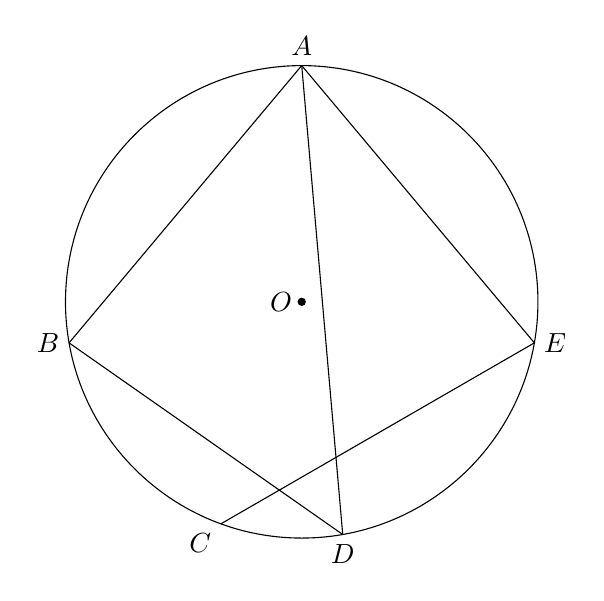
\begin{tikzpicture}[scale=1.5]
    % Define coordinates based on the visual layout
    \coordinate (O) at (0,0);
    \coordinate (A) at (90:2);      % Top
    \coordinate (B) at (190:2);     % Left
    \coordinate (C) at (250:2);     % Bottom Left
    \coordinate (D) at (280:2);     % Bottom
    \coordinate (E) at (350:2);     % Right

    % Draw the circle
    \draw (O) circle (2);

    % Draw the center point and label
    \fill (O) circle (1pt);
    \node[left] at (O) {$O$};

    % Draw existing lines from the original image
    \draw (A) -- (B);
    \draw (A) -- (E);
    \draw (B) -- (D);
    \draw (E) -- (C);

    % Instruction: Connect point A and point D, draw solid line segment AD
    \draw (A) -- (D);

    % Draw labels
    \node[above] at (A) {$A$};
    \node[left] at (B) {$B$};
    \node[below left] at (C) {$C$};
    \node[below] at (D) {$D$};
    \node[right] at (E) {$E$};
\end{tikzpicture}

\end{document}
